\documentclass{article}
\usepackage{pdfpages}
\usepackage{geometry}
\usepackage{algorithm}
\usepackage{algorithmic}
\usepackage{amsmath}
\usepackage{graphicx}
\usepackage{inputenc}
\usepackage{ctex}
\usepackage{listings}
\usepackage{url}
\usepackage{color}
\usepackage{titlesec}
\usepackage{booktabs}


\lstset{
    basicstyle=\tt,
    keywordstyle=\color{blue}\bfseries,
    identifierstyle=\color{purple},
    commentstyle=\color{gray},
    showstringspaces=false,
    numbers=left, numberstyle=\it, stepnumber=1, numbersep=5pt,
    frame=shadowbox,
    framexleftmargin=4mm,
    rulecolor=\color{gray},
    rulesepcolor=\color{gray},
    backgroundcolor=\color{white}
}
\geometry{a4paper,left=3cm,right=3cm,top=2cm,bottom=2cm}


\title{基于遗传算法的机器作曲}
\author{第4题第1组}
\date{2023年12月}
\begin{document}
\pagenumbering{arabic}
\maketitle

\begin{abstract}
我们使用遗传算法进行机器作曲。指导进化方向的
适应度函数(fitness function)包括两种模式,即基于乐理特征的适应度函数,以及增加了基于卷积神经网络评分的适应度函数。
我们实现了包括倒影,移调变换在内的多种变异方式。最终,我们的遗传算法模型从随机序列片段开始,能够生成质量较高的乐曲。

\begin{center}
    \textbf{关键词:遗传算法,适应度函数,机器作曲,卷积神经网络}
\end{center}
\end{abstract}

\section{引言}
随着人工智能的快速发展,它在各个领域展现出了巨大的潜力,其中也包括音乐创作。
音乐作为一种艺术形式,一直以来都是人类创造力的重要表达方式。
随着科技的发展,人们开始思考如何利用人工智能技术来创作音乐,以拓展音乐的边界。
遗传算法作为一种模拟自然进化过程的计算方法,被引入到音乐创作中,为机器作曲提供了一种创新的思路。
通过模拟基因的遗传、交叉和变异过程,遗传算法可以生成多样性的音乐片段,并通过选择和进化策略逐步优化,最终形成完整的音乐作品。
基于遗传算法的机器作曲为音乐创作提供了一种全新的方式,突破了传统音乐创作的限制,创造出更加多样化和创新的音乐作品。
通过遗传算法的优化过程,遗传算法模型能够自动化生成音乐,减轻了音乐人的创作负担,提高了音乐创作的效率。
此外,我们的项目还为音乐爱好者和听众提供了更多选择,让他们能够欣赏到更多种类的音乐作品,丰富了人们的音乐体验。

本项目是基于遗传算法的机器作曲项目,旨在探索人工智能在音乐领域的应用,为音乐创作带来全新的可能性。
通过模拟进化过程,该项目能够生成独特而优美的音乐作品,为人们带来美妙的听觉体验。
我们探讨了基于遗传算法的机器作曲方法,并就其在音乐创作领域的应用进行深入研究与分析;
通过对遗传算法的原理和机制进行介绍,并结合音乐理论、计算机科学和人工智能等领域的知识,研究了如何利用遗传算法创作出高质量的音乐作品。
我们对遗传算法的参数设置、适应度函数设计以及遗传过程的优化等关键问题展开了深入的讨论,以期为机器作曲技术的进一步发展提供新的思路和方法。

\section{遗传算法}
遗传算法(Genetic Algorithm,GA)是一种启发式优化算法,灵感源自达尔文的进化理论。
它模拟了生物进化的过程,通过群体内个体之间的选择、交叉和变异等操作来搜索和优化解空间中的解。
这种算法常用于解决复杂的优化问题,尤其是那些搜索空间巨大且没有明显规律的问题。

具体来说,遗传算法包括初始化种群,适应度评估,选择,交叉,变异,替换等步骤。
首先,遗传算法开始于生成一个初始的种群,这个种群由候选解组成。
候选解通常由基因组成,每个基因代表解空间中的一个参数或变量。
初始种群是随机生成的,通常包含多个个体。
对每个个体,需要定义一个适应度函数来评估其优劣程度。
适应度函数用于量化个体解的质量,是优化问题的目标函数。
通过适应度评估,可以确定个体在解空间中的位置和潜在的解决方案。
在选择阶段,根据适应度函数的评估结果,从当前种群中选择一部分个体作为繁殖的父代。
通常,适应度较高的个体被选中的概率较大。
选定的父代个体进行基因信息交换,模拟生物进化中的交叉过程。
通过交叉,父代个体之间的基因片段互换,产生新的个体。这个过程有助于保留种群中有价值的基因信息。
新生成的个体可能会经历变异过程,即在个体基因中引入随机变化。
变异操作有助于维持种群的多样性,防止陷入局部最优解。通常,变异率很低,只对少数个体进行变异。
经过交叉和变异产生的新个体将部分或全部替换掉旧的个体,形成下一代种群。
这个过程通常称为生成子代或新种群。
以上步骤将持续迭代,生成新的个体并更新种群,直到满足停止条件,例如达到最大迭代次数或解的精度满足特定要求。
下图展示了遗传算法的伪代码。



为了将遗传算法应用于我们的项目,我们首先利用随机生成的片段作为初始种群,
我们实现了基于乐理特征的适应度函数,以及基于卷积神经网络的适应度函数来评估片段的质量。
在选择阶段,我们依据当前种群个体的适应度函数评分得到与之负相关的作为繁殖父代的概率,并依此概率进行随机抽取下一代个体。
我们实现了多种变异方式,以增加遗传算法演化的多种可能性。重复迭代上述过程,我们的遗传算法模型最终具有输出较高质量乐曲的能力。


\begin{algorithm}
    \caption{Genetic Algorithm}
    \begin{algorithmic}[1]
    \STATE Initialize population:
        \STATE Create a population with random individuals
    \STATE Evaluate fitness of individuals:
        \STATE Calculate fitness value for each individual in the population
    \REPEAT
        \STATE Select parent individuals:
            \STATE Use selection algorithm to choose individuals as parents
        \STATE Perform crossover:
            \STATE Apply crossover operation to selected parent individuals to generate new individuals
        \STATE Perform mutation:
            \STATE Apply mutation operation to the new individuals
        \STATE Evaluate fitness of new individuals:
            \STATE Calculate fitness value for the newly generated individuals
        \STATE Select surviving individuals:
            \STATE Choose which individuals survive and form the new population
    \UNTIL{termination condition is met}
    \STATE \textbf{return} Best individual or best solution when termination condition is reached
    \end{algorithmic}
    \end{algorithm}


\section{适应度函数}
适应度函数作为遗传算法的核心,直接决定了遗传算法模型如何选择遗传过程中的乐曲。
选择适应度函数的主要挑战在于确定如何量化乐曲的质量以确定其遗传的概率。
然而,音乐本身具有主观性,难以挖掘绝对客观的量化指标评价任意乐曲的质量。
为了使遗传算法模型尽可能客观地评价生成的乐曲质量,我们调查并尝试了诸多基于乐理特征的适应度算法,
将适应度函数定义为各个乐理特征评价的加权。

另外,我们利用卷积神经网络模型(CNN),收集了乐曲数据集以训练一个乐曲的分类器,
并对于给定的乐曲将分类器的预测结果作为乐曲质量的另一个评价准测。

综合以上两种方法,用$\lambda$表示权重, $f$表示基于不同乐理特征的适应度函数,
更高的适应度函数评分意味着更低的乐曲质量,使乐曲在遗传中的贡献越小。
$mode$表示是否采用卷积分类器结果,$\tau$表示分类器预测结果,我们的模型适应度函数为

\begin{align}
    f(x)=\sum_{i=1}^{n} \lambda_i \cdot f_i(x) + \lambda_{CNN} mode \cdot \tau(x)
\end{align}


\subsection{基于乐理特征的适应度函数}
我们参考了\cite{article1}\cite{article2},选择实现了其中5个最基本的适应度函数。
我们认为,基于乐理特征的适应度函数应该遵循音程协和,调性一致的准则。
所以我们首先确定基于音程协和性的适应度函数,以及基于调性一致性的适应度函数,
使遗传算法模型倾向于保留具有更多协和音程,以及更具有自然大调调性的乐曲。

此基础上我们考虑了音乐音符的多变性。为了防止遗传算法总是收敛于一列等音序列(尽管这也被定义为协和且具有良好的调性),
或者只包含最协和的纯一度与纯八度音程的序列,我们考虑了基于音程的自相似度,以及基于音类分布的适应度函数,
使遗传算法模型倾向于保留使用了更多种类音程,以及更多种类音类的乐曲。

最后,我们考虑了乐曲节奏的多变性,在遗传过程中引入了休止与延长变异,
并使用基于节奏相似度的适应度函数来评价乐曲的节奏质量,使得生成结果在节奏上有别于初始随机种子的八分音符序列节奏。

\subsubsection{基于音程协和性的适应度函数}
基于各音程的性质,我们对所有相邻音程的协和性进行评分(跳过休止符或者延音符)。
为简单起见,对音程定义进行简化,只考虑两个音级实际相差的半音数,而忽略音名间的度数。具体取值如表1所示。

\begin{table}[htbp]
    \centering
    \caption{音程协和性的评分}
      \begin{tabular}{ccc}
      \toprule
      音程种类 & 音程 & 评分 \\
      \midrule
      完全协和 & 纯一、四、五、八度 & 1 \\
      不完全协和 & 大小三度、大小六度 & 2 \\
      二度 & 大小二度 & 3 \\
      七度 & 大小七度 & 3 \\
      超八度 & 超过八度的音程 & 5 \\
      \bottomrule
      \end{tabular}
  \end{table}%

根据该规则,对某一遗传个体的音程进行评分,根据评分结果计算出音乐个体每小节的音程平均得分,如式(2)所示。
\begin{align}
    a_i = \frac{1}{n_i}\sum_{j=1}^{n_i} x_{i,j}
\end{align}

式中,$x_{i,j}$表示第$i$小节的第$j$个音程,$n_i$表示第$i$小节相邻两个音符的音程数目(跳过休止符和延音符),
$a_i$表示第$i$小节的平均音程得分。接着计算音乐个体每一小节的音程得分方差,如式(3)所示。
\begin{align}
    b_i ^2 = \frac{1}{n_i}\sum_{j=1}^{n_i} (x_{i,j}-a_i)^2
\end{align}

式中,$b_i ^2$表示第$i$小节的音程得分方差。

随后,给出参考音乐的每小节平均音程得分$\mu$和音程得分方差$\sigma$,
并定义两个适应度函数,如式(4)(5)所示。
\begin{align}
    f_1=\sum_{i=1}^{n}\zeta_i | \mu_i-a_i |\\
    f_2=\sum_{i=1}^{n}\eta_i | \sigma_i ^2-b_i ^2 |
\end{align}

式中,$f_1$、$f_2$分别表示基于音程得分均值和方差的两个适应度函数,
$\zeta_i$表示第$i$小节的音程得分均值的影响权重,
$\eta_i$表示第$i$小节的音程得分方差的影响权重。

\subsubsection{基于调性一致性的适应度函数}

这一适应度函数使模型倾向于选择符合自然大调调性的乐曲。
但是,由随机种子开始的遗传过程并不保证收敛到某个特定的自然大调,因此我们考虑了多种调性。
对于所有12个自然大调,我们分别统计不同调性的调内音符出现频率,
并将出现频率最高的调定义为该个体的调性,对应的频率用于衡量调性一致性,如式(11)(12)所示。
\begin{gather}
    Key_j(I) = \frac{|K_j|}{|I|}\\
    Tonality(I) = \max_j Key_j(I)-\frac{1-\max_j Key_j(I)}{n-1}
\end{gather}

其中$K_j$表示属于第$j$个调性的音符数量($j=1$表示C自然大调,$j=2$表示\#C大调以此类推),$Key_j$表示第j个调性的调内音出现频率,
$n$表示遗传个体的音列长度,即$|I|$,
Tonality(I)表示调性一致性,与出现频率最高的调性对应的频率有关,调性一致性越高,该调性的调内音出现频率也就越高。
这里同样用3.1.2的式(8)来得到基于调性一致性的适应度函数$f_{Tonality}$。

\subsubsection{基于音程自相似度的适应度函数}

基于音程自相似度的适应度函数使模型倾向于选择包含更多种类的音程,以避免算法收敛到只包含完全协和音程的个体上。
这里的音程做了与3.1.1相同的简化。定义音程自相似度表示不同类的音程在音乐中出现的频率占比的均值,
计算公式如式(6)(7)所示。
\begin{gather}
    SelfSimilarity(I)=\max(1, \frac{2\mu}{|I|})\\
    \mu=\frac{1}{|S|}\sum_{s\in S} count_s(I)
\end{gather}

式中,$SelfSimilarity(I)$表示某一遗传个体$I$的音程自相似度值,
$|I|$表示该遗传个体的音列长度,$S$表示$I$中所有音程的种类集合,
$|S|$表示音程的种类数目,$s$表示某类出现在$I$中的音程,如纯八度,
$count_s(I)$表示音程$s$在$I$中出现的次数,$\mu$表示不同类的音程在$I$中出现的次数的均值

随后,我们将自相似度与\cite{article1}中的推荐值来衡量遗传个体在这一指标下的质量,得到最终的适应度得分,如式(8)(9)所示。
\begin{gather}
    FeatureScore(t,e(I))=\frac{1}{\frac{-1}{(x(t)-t)^2}(e(I)-t)^2+1}\\
    x(t)=\left\{\begin{matrix}
        1,\ if\ t<0.5\\ 
        0,\ if\ t\geq 0.5
        \end{matrix}\right.
\end{gather}

式中,$t$表示参考音乐的标准值,$e(I)$表示遗传个体在特征$e$上表现的值,
这里的$e(I)$特指$SelfSimilarity(I)$,$FeatureScore(t,e(I))$表示基于特征$e$的适应度函数$f_e$,越小说明该遗传个体表现的越好。
据此得到基于音程自相似度的适应度函数$f_{SelfSimilarity}$。

\subsubsection{基于音类分布的适应度函数}

音类分布用于衡量该遗传个体音符对应的音类分布情况,计算公式如式(13)所示。
\begin{gather}
    PitchDistribution(I)=\frac{\frac{n-\max_j P_j(I)}{11}\cdot 12}{n}
\end{gather}

式中,$P_j(i)$表示$I$中属于音类$j$的音符个数,音类分布$PitchDistribution(I)$越大,表示该个体中音符更均匀地分布在各个音类当中。
同样用3.1.2的式(8)来得到基于音类分布的适应度函数$f_{PitchDistribution}$。

\subsubsection{基于节奏相似度的适应度函数}

节奏相似度衡量的是不同小节之间的节奏相似程度,我们认为节奏相似度越高的音乐会更加动听。计算公式如式(14)所示。
\begin{align}
    RhythmSimilarity(I) = \frac{2}{nm(m-1)}\sum_{i=1}^{m-1} \sum_{i'=i+1}^{m} \sum_{j=1}^{n} |r_{i,j}-r_{i',j}|
\end{align}

其中$r_{i,j}$表示第$i$小节第$j$个音符的类型,$m$表示小节数,这里我们将休止符、延长音、八分音符分别对应$r$=0、1、2。
因此,$RhythmSimilarity(I)$越大,意味着节奏相似度越高,
这里我们直接将$RhythmSimilarity(I)$作为基于节奏相似度的适应度函数$f_{RhythmSimilarity}$

\subsection{基于卷积神经网络的适应度函数}
神经网络模型已经被广泛地应用于分类任务。其中,基于循环神经网络(RNN)以及此基础上的LSTM模型在处理序列数据上表现出优越的性能。
但我们认为在这一任务中,较短的向量(32位八分音符向量)与较小的数据空间(每个音符只能在接近两个八度范围内取离散值)
使得乐曲模态数据中蕴含的序列信息相比于传统的文本模态更少,在较大模型容量下更容易产生数据过拟合的现象。

另一方面,动听乐曲的特征包括片段的重复,音程的协和,调性的一致,在一定程度上都可以理解为特定的局部模式特征。
例如,音程的协和性可以理解为较小感受野范围内的模式特征,片段的重复与调性的一致可以理解为较大范围的模式特征。
基于这一观点,我们设计实现了卷积神经网络作为乐曲的分类器。

我们收集了超过200首流行乐曲数据作为正样本,并生成了相当数量的随机片段作为负样本,训练了卷积网络模型。
并在测试集上获得了超过90\%的准确率。
在遗传算法中,我们使用卷积网络模型的负样本预测概率值作为适应度函数评分,具体为

\begin{align}
    \tau(x) = softmax_{-}(logit_{+}, logit_{-}) = \frac{e^{logit_{-}}}{e^{logit_{+}} + e^{logit_{-}}}
\end{align}

然而,我们在实验中发现,这一分类模型并不能很好地指导遗传算法的进行。
由于训练数据量过小,数据的过拟合现象仍然存在,模型输出的概率预测值倾向于接近0,1二值。
因此,我们尝试了直接使用模型的logit输出作为适应度函数值,并将其线性变换到0-1区间内,使得在训练过程中
该项适应度函数值平稳变化,且与其他项保持一致的数量级,即最终的适应度函数为

\begin{align}
    \tau(x) = W(0.5 + \frac{logit_{-}}{2 \cdot Bound})
\end{align}

其中$W(x) = \min(\max(x, 0), 1)$为0-1窗口函数,保证适应度函数取值位于0-1之间

\section{实验}
\subsection{变异}
我们参考了\cite{article2}中的建议,在遗传算法中没有采用交叉遗传(crossover)的方式来产生新一代种群,
而是完全基于父代的变异以产生新一代种群。其中的主要原因是个体的取值空间小,对个体进行截断重组的效果并不好;
而且,在给定简单适应度函数的情况下,基于变异得到的最优解难以通过交叉遗传改进。

因此,我们结合\cite{article2}以及任务要求中的变异种类,选择实现了六种变异,具体如下。
移调变换,将随机一小节整体在上下三度内移动;倒影变换,将随机一小节做倒影变换;
八度变异,将随机一个音符上移或下移八度;音符变异,将随机一个音符在上下五度范围内移动;
休止变异,将随机一个音符休止;延长变异,将随机一个音符延长。
由于我们限制了所有的音符位于$\text{F3-G5}$音域中,当变异导致音符越出这一音域,
我们发现简单地将音符设定为音域边界会引入系统性偏差,导致结果中的边界音符(F3, G5)显著增加;
因此,对于这种情况,我们将越界音符随机地设定为音域中的任意音符以提高算法的效率。

由于我们在遗传算法中没有使用交叉遗传,因此最终结果完全是由初代种群经历若干代个人变异得到的,
变异概率的绝对值与相对值,以及遗传算法的种群规模和迭代数量将显著影响算法生成的乐曲的质量。
我们采取的具体参数将在下一节中给出。

\subsection{遗传算法超参数}
遗传算法中的超参数包括,变异的种类概率$p$, 最大种群数量 $M$, 算法迭代的最大次数 $N$。我们没有设定终止算法的适应度阈值,因此算法只会在迭代最大次数后终止。
另外的超参数包括,各适应度函数权重$\lambda$以及CNN评分参数$Bound$。我们的最终超参数设定为$p = [0.95, 0.015, 0.015, 0.005, 0.005, 0.005, 0.005]$,
分别对应无变异与六种变异的概率,$M=15000, N=300$。各个适应度函数的权重依次为$\lambda = [0.5, 0.2, 0.1, 2, 2]$, $\lambda_{CNN}=5. Bound = 800$

\subsection{模型训练集,测试集}
为了训练能够区分高质量与低质量乐曲的CNN分类器,我们人工选取了超过200个流行乐曲片段并转换为我们采用的音符编码,
作为训练集与测试集中的正样本。(如图所示)另外,我们随机生成了相同数量的随机片段作为负样本。
我们发现,尽管在训练集上训练出的模型能够在测试集上表现出超过90\%的准确率,但是在遗传算法中对遗传方向的指导仍然是有限的。
为此,我们将数据集负样本替换为初步实验时生成的较低质量的乐曲。
同样模型能够在测试集上表现出优秀性能,但负样本替换为这些较低质量片段后模型对遗传算法的指导作用显著增加,
这体现在模型给出的适应度评分在整个遗传算法迭代过程中表现出了显著下降趋势。

\section{结果分析}
可以在 \url{https://github.com/XHZhao2003/Composer_GeneticAlgorithm} 查看我们的详细实验结果以及代码。

我们利用五种适应度函数,以及添加CNN模型分别进行了五十次遗传算法实验,每次实验算法将输出十首适应度评分最低的片段。
我们最终选取了十首具有代表性的片段作为最终结果,下图展示了其中的部分片段。

\begin{figure}[htbp] 
    \centering
    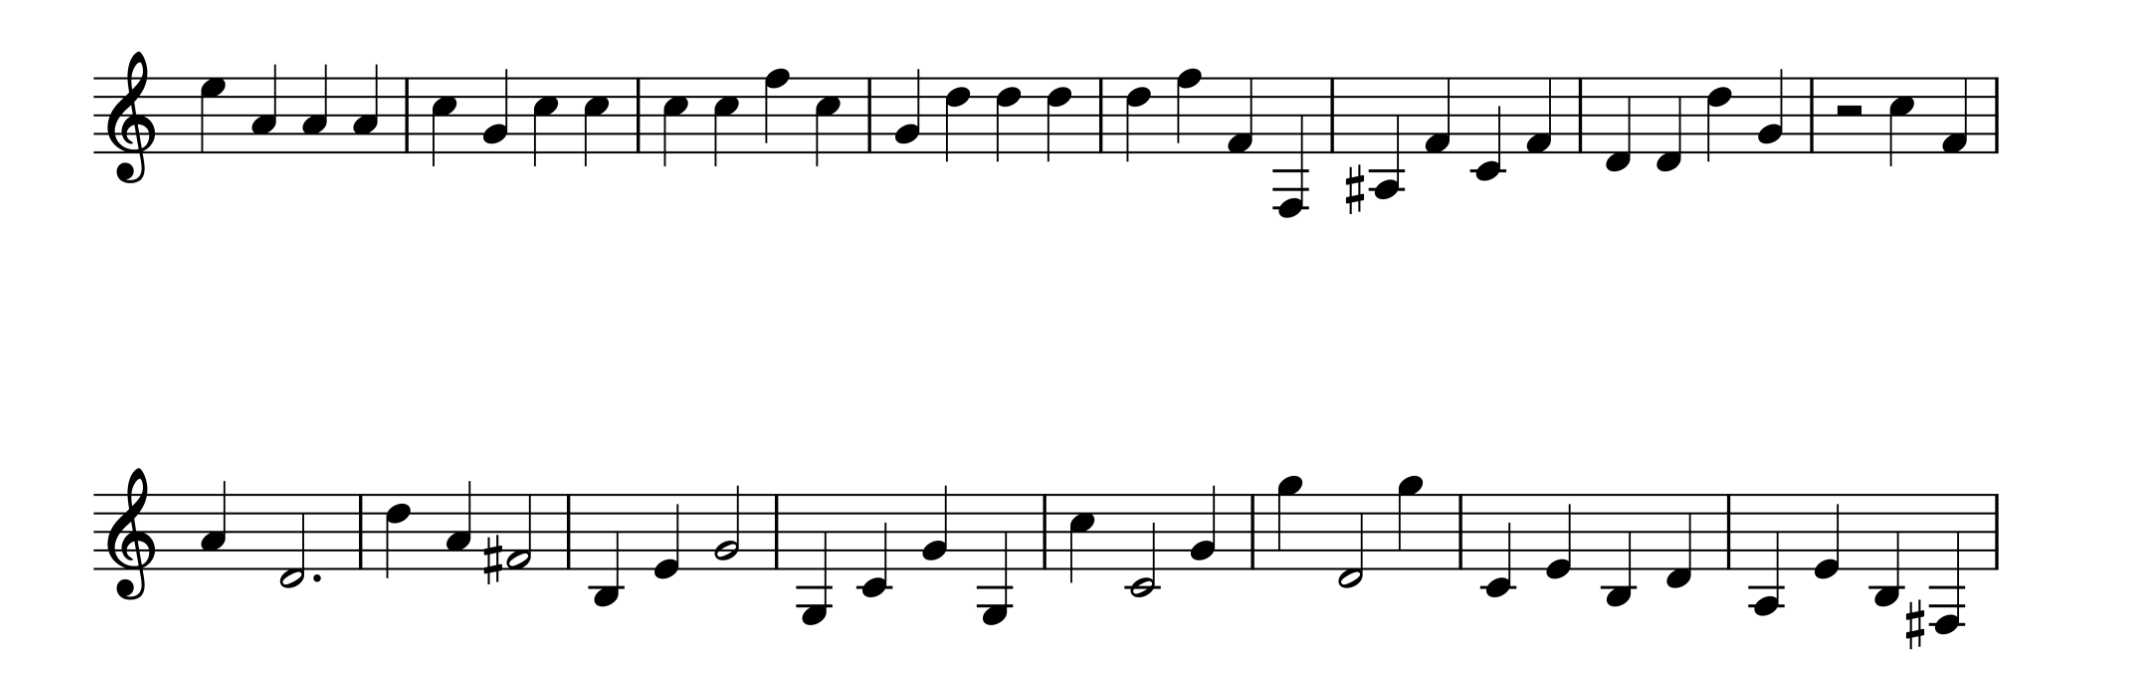
\includegraphics[width=0.7\textwidth]{result1.png} 
    \caption{Basic适应度下的输出} 
\end{figure}

\begin{figure}[htbp] 
    \centering
    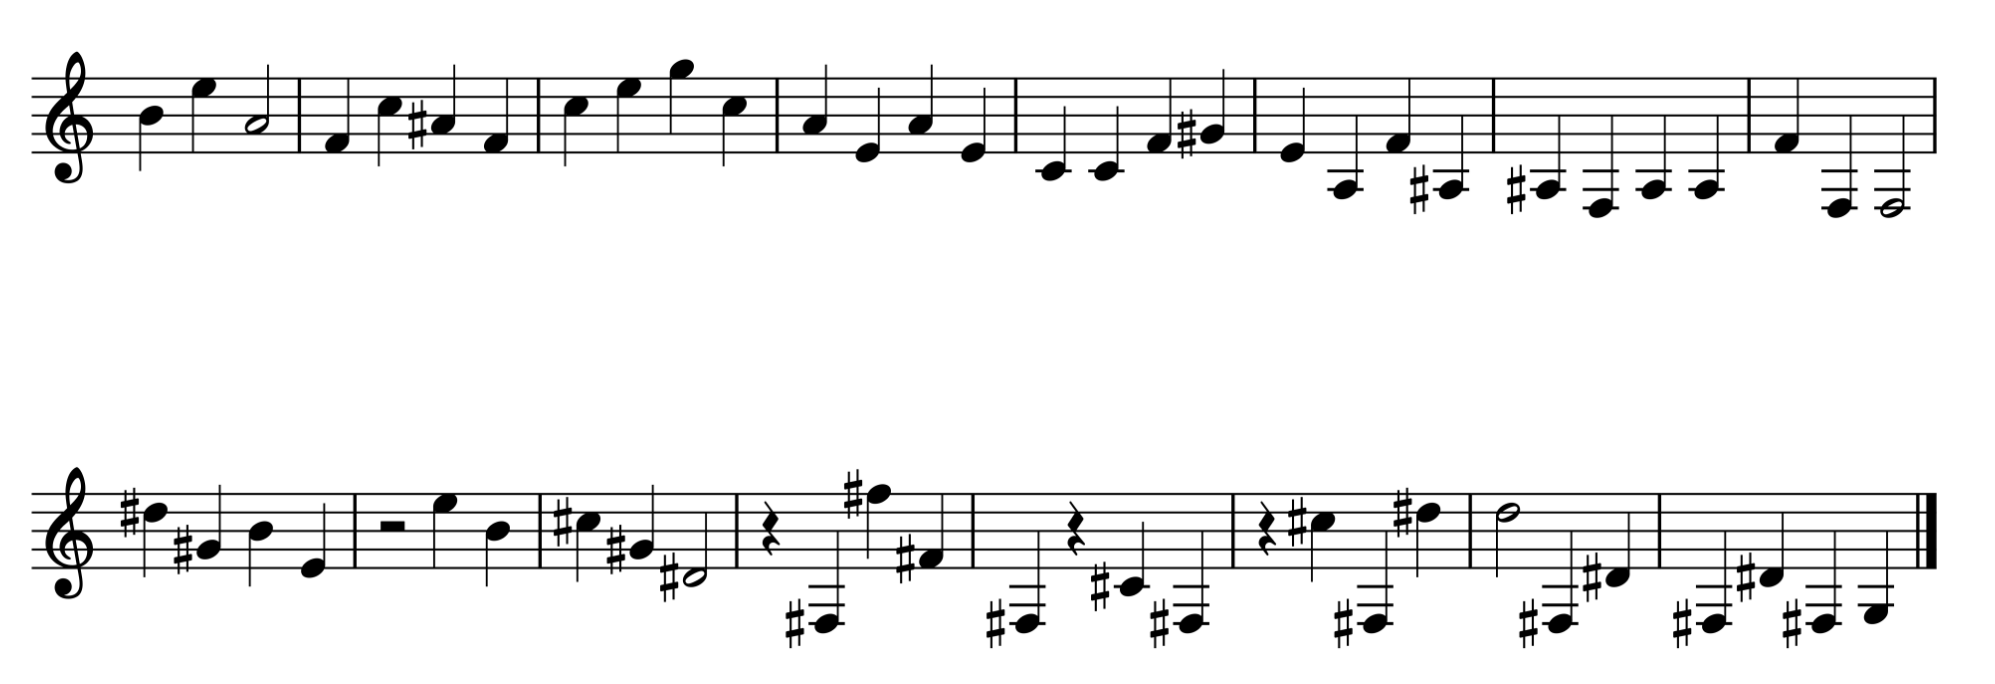
\includegraphics[width=0.7\textwidth]{result2.png} 
    \caption{增加CNN适应度下的输出} 
\end{figure}



总体来说,在我们的参数设定下,遗传算法模型能够生成比较和谐动听的乐曲片段。不同的参数设定会导致模型具有不同的性能。
例如在给定变异概率的情况下,更多的迭代次数有利于模型收敛到较低的适应度值,从而产生质量更高的乐曲;
在给定迭代次数的情况下,较低的变异概率将导致降低算法收敛的速度从而影响算法效率,
而过高的变异概率将遗传过程中随机得到的较高质量的乐曲难以在下一代中保持,从而也严重影响了算法的效率。

此外,我们深入分析了我们引入的卷积神经网络模型在遗传算法中的作用。
在我们的初步尝试后我们认为,利用流行歌曲片段作为正样本随机片段作为负样本得到的卷积模型对遗传算法的贡献很小
主要是因为以下两个因素:
第一,模型的训练数据与遗传算法数据间存在较大偏差。模型的训练数据包括收集的流行乐曲片段与随机片段,
而遗传算法中模型的输入为遗传中的个体,与训练集存在明显的数据偏移,导致模型无法泛化到遗传种群上。
第二,模型的训练任务被建模为分类任务而非回归任务,这意味着模型的输出是离散值而非离散值。

考虑到上述的数据偏移因素使得模型的概率输出并不可信,我们尝试了将任务由二分类细化为三分类以及多分类,
将遗传算法模型(不含CNN模块)的输出作为中间类别样本,但这样做只得到了微小的改进。
我们认为,使用回归模型作为非乐理特征的评分器是更合适的,但是这为数据收集带来了新的挑战。
一方面,我们难以定义与收集到质量介于流行音乐与随机片段之间的音乐形式片段;
另一方面,人工的数据标注过程仍然将引入主观性,这一步骤仍然需要额外的讨论与论证。
但一种可能可行的替代方式是,使用客观的乐理标准对片段进行标注评价,从而使在遗传算法中引入回归模型模块成为可能。

\section{成员贡献}
姚昕蒴:收集与清洗数据,撰写实验报告

孙鹏:适应度函数的文献调研与实现工作,撰写报告中的对应部分

赵潇晗:遗传算法与卷积神经网络的实现与实验工作,数据清洗与转换,撰写报告中的对应部分

聂羽佳:收集与清洗数据,构建训练集与测试集

孙荣荣:数据的收集与处理,撰写实验报告

闫宏远:数据收集处理,结果的可视化工作


\begin{thebibliography}{2}
    \bibitem[1]{article1}Murray S, Ventura D. Algorithmically flexible style composition through multi-objective fitness functions[C] Proceedings of the AAAI Conference on Artificial Intelligence and Interactive Digital Entertainment. 2012, 8(4): 55-62
    \bibitem[2]{article2}Matić D. A genetic algorithm for composing music[J]. Yugoslav Journal of Operations Research, 2010, 20(1): 157-177.
\end{thebibliography}

\end{document}
